\documentclass{beamer}
\usepackage[italian]{babel}
\usepackage[justification=centering]{caption}
\usepackage{makecell}
\usepackage{adjustbox}
\usepackage{subcaption}
\usepackage{booktabs}
\usepackage{multirow}

\usefonttheme[onlymath]{serif}
\definecolor{darkred}{rgb}{0.8,0,0}
\usetheme{Szeged}
\usecolortheme{beaver}
\setbeamertemplate{navigation symbols}{}
\setbeamertemplate{footline}[frame number]
\setbeamercolor{caption name}{fg=darkred}
\setbeamercolor{description item}{fg=darkred}
\setbeamercolor{block title}{fg=darkred}
\setbeamertemplate{itemize item}{\color{darkred}$\blacktriangleright$}
\defbeamertemplate{description item}{align left}{\insertdescriptionitem\hfill}

\title{A Self-Supervised Attribution Method for Explaining Neural Networks}
\author{}
\institute{}
\date{}

\def\M{{\ensuremath{\mathbf{M}}}}
\def\S{{\ensuremath{\mathbf{S}}}}
\def\L{{\ensuremath{\mathcal{L}}}}
\def\x{{\ensuremath{\mathbf{x}}}}


\begin{document}

{
    \setbeamertemplate{footline}{}
    \begin{frame}
        \title{}
        \begin{center}
            \vspace*{3em}
            {
                \color{darkred}\LARGE
                A Self-Supervised Attribution Method for Explaining Neural Networks
            }

            \vspace*{2em}
            \small
            \begin{minipage}{0.49\linewidth}
                \raggedright
                Supervisor:\\
                Prof. Paolo Torroni \\
                Co-supervisor: \\
                Prof. Akiko Aizawa
            \end{minipage}
            \begin{minipage}{0.49\linewidth}
                \raggedleft
                Candidate:\\
                Tian Cheng Xia
            \end{minipage}

            \vspace{2em}
            \footnotesize
            Master's Degree in Artificial intelligence \\
            Alma Mater Studiorum $\cdot$ Università di Bologna
        \end{center}
    \end{frame}
    \addtocounter{framenumber}{-1}
}



\begin{frame}
    \frametitle{Motivation}
    \textbf{Attribution methods} Methods that produce an explanation by scoring input features.\\[1em]

    Existing attribution methods:
    \begin{itemize}
        \item Require tuning method-specific hyperparameters.
        \item Need to perform multiple iterations or do backpropagation at inference time.
    \end{itemize}
\end{frame}


\begin{frame}
    \frametitle{Intuitive Idea}
    
    \textbf{Assumption} A good attribution map should only highlight elements that, if isolated from the input, allow the model to predict the same outcome.

    \begin{itemize}
        \item Pair the existing model with a separate module to produce attribution maps.
        \item The new module is trained to produce attribution maps that preserve the capabilities of the original model, when used as a weight of the input.
    \end{itemize}
        
    \[
        \min_{\S \in [0, 1]^{N}} \left\Vert f(\x) - f(\x \otimes \S) \right\Vert + \gamma \left\Vert \S \right\Vert
    \]
\end{frame}


\begin{frame}
    \frametitle{Moving to Neural Networks}
    
    When working with neural networks, we can define the problem in terms of loss function:
    \[
        \min_{\S \in [0, 1]^{N}} \left\Vert f(\x) - f(\x \otimes \S) \right\Vert + \gamma \left\Vert \S \right\Vert
    \]
    \[\Downarrow \]
    \[
        \min_{\S \in [0, 1]^{N}} \L(\x \otimes \S; f) + \gamma \left\Vert \S \right\Vert
    \]
\end{frame}


\begin{frame}
    \frametitle{Architecture}

    The scoring module works in the embedding space of the target model and produces the attribution map with a single forward pass. \\[1em]

    To guide scores prediction, the head of the scorer is composed of:
    \begin{itemize}
        \item \textbf{ReLU} Cuts off negative scores (i.e., not relevant),
        \item \textbf{Sigmoid} Stabilizes scores into $[0.5, 1]$,
        \item \textbf{Rescale} Ensure the highest score is $1$ and lowest is $0$.
    \end{itemize}

    \begin{figure}[H]
        \centering
        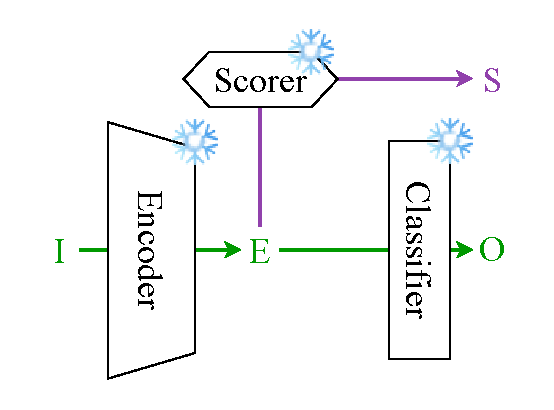
\includegraphics[width=0.45\linewidth]{../thesis/img/inference.pdf}
    \end{figure}
\end{frame}


\begin{frame}
    \frametitle{Training Problem (1/2)}
    {
        \small
        \[
           \begin{aligned}
                \L(\x, \S; f) =\,\, &\L_\text{task}(\x \otimes \S; f) & \text{Preserve original loss} \\
                &+ \gamma_1 \left( \frac{1}{\vert \S \vert} \sum_i^{\vert S \vert} s_i \right)^2 & \text{Encourage sparsity} \\
                &+ \gamma_2 \frac{1}{\vert \S \vert} \sum_i^{\vert S \vert} (s_i \cdot (1-s_i))^2 & \text{Encourage binary-like scores} \\
            \end{aligned}
        \]
    }

    \begin{figure}[H]
        \centering
        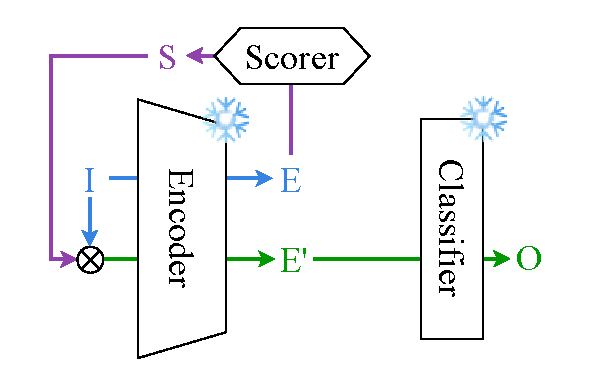
\includegraphics[width=0.45\linewidth]{../thesis/img/idea.pdf}
    \end{figure}
\end{frame}


\begin{frame}
    \frametitle{Training Problem (2/2)}
    
    We can self-calibrate the hyperparameters $\gamma_1$ and $\gamma_2$ during training:
    \[
    \gamma = \texttt{clip}\left\{ \frac{1}{\L_\text{task}(\x \otimes \S; f) - \L_\text{task}(\x; f) + \varepsilon}, [0, 1] \right\}
    \]
    \textbf{Intuitive idea} When the distance between the loss functions of the weighted and original input is:
    \begin{itemize}
        \item Large: the penalty terms are less important.\\
        $\Rightarrow$ preserve the original capabilities first. 
        \item Small: reintroduce the penalties.\\
        $\Rightarrow$ can focus back to attribution maps. 
    \end{itemize}
\end{frame}


\begin{frame}
    \frametitle{Modalities}
    Depending on the type of data, the scorer can be implemented as:
    \begin{itemize}
        \item \textbf{Text} Small transformer encoder.
        \item \textbf{Image} U-Net-style upsampling branch.
        \item \textbf{Multimodality} One scorer for each modality.
    \end{itemize}
\end{frame}


\begin{frame}
    \frametitle{Datasets}
    
    \begin{table}[H]
        \centering
        \scriptsize
        \def\arraystretch{1.0}
        \makebox[\linewidth][c]{%
            \begin{tabular}{llp{6cm}}
                \toprule
                \textbf{Modality} & \textbf{Name} & \textbf{Task} \\
                \midrule
                \multirow{3}{*}{Text} & Tweet Sentiment & Sentiment analysis, short texts. \\ 
                                    & IMDB                       & Sentiment analysis, long texts. \\
                                    & LIAR                       & Fact checking. \\
                \midrule
                \multirow{3}{*}{Image} & MNIST      & Image classification, grayscale, low-resolution. \\ 
                                    & CIFAR-10   & Image classification, colored, low-resolution. \\ 
                                    & Imagenette & Image classification, colored, high-resolution. \\ 
                \midrule
                \multirow{3}{*}{Multimodal} & Flickr8k & Image-caption alignment. \\ 
                                            & Hateful Memes & Hateful content detection. \\ 
                                            & SNLI-VE & Visual entailment. \\ 
                \bottomrule
            \end{tabular}
        }
    \end{table}
\end{frame}


\begin{frame}
    \frametitle{Metrics}
    
    \textbf{Faithfulness} Is the explanation reflecting the underlying process?
    \begin{itemize}
        \item Average drop,
        \item Deletion AUC.
    \end{itemize}
    \vspace{1em}
    \textbf{Clarity} Is the explanation visually appealing?
    \begin{itemize}
        \item Complexity,
        \item Sparsity.
    \end{itemize}
\end{frame}


\begin{frame}
    \frametitle{Baselines}
    
    \begin{itemize}
        \item Saliency,
        \item Guided Backpropagation,
        \item Integrated Gradients,
        \item DeepLIFT,
        \item DeepLIFT-SHAP,
        \item Gradient-SHAP.
    \end{itemize}
\end{frame}


\begin{frame}
    \frametitle{Results}
    \framesubtitle{Quantitative (1/4)}
    
    \begin{itemize}
        \item Saliency is the method with the best Complexity and Sparsity results.
        \item The other baselines achieve the best results in terms of Average Drop and Deletion AUC.
        \item Our method balances faithfulness and clarity.
    \end{itemize}
\end{frame}

\begin{frame}
    \frametitle{Results}
    \framesubtitle{Quantitative (2/4)}
    
    \begin{figure}[H]
        \centering
        \begin{subfigure}[c]{0.3\linewidth}
            \centering
            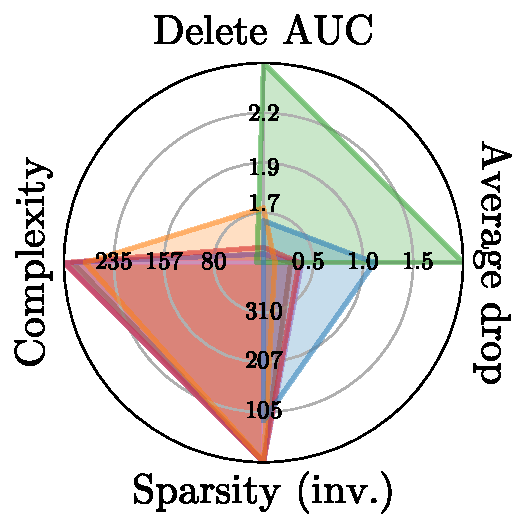
\includegraphics[width=0.9\linewidth]{../thesis/img/radar-tweet.pdf}
            \caption{Tweet Sentiment}
        \end{subfigure}
        \begin{subfigure}[c]{0.3\linewidth}
            \centering
            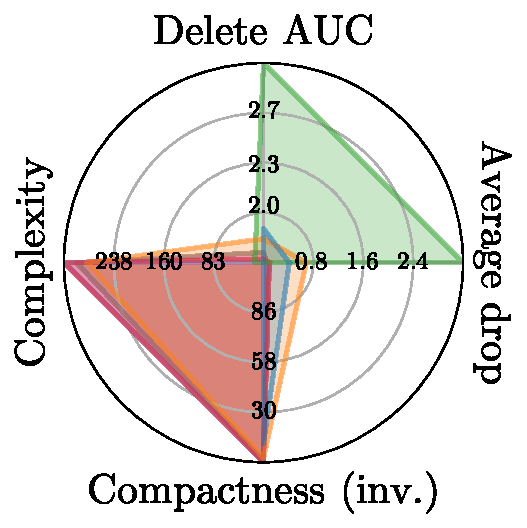
\includegraphics[width=0.9\linewidth]{../thesis/img/radar-imdb.pdf}
            \caption{IMDB}
        \end{subfigure}
        \begin{subfigure}[c]{0.3\linewidth}
            \centering
            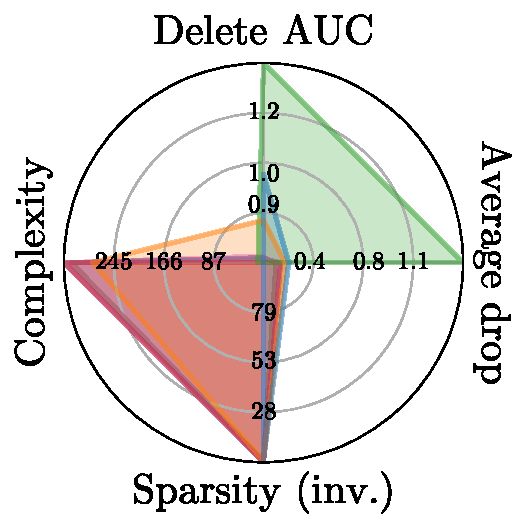
\includegraphics[width=0.9\linewidth]{../thesis/img/radar-politifact.pdf}
            \caption{LIAR}
        \end{subfigure}
        \begin{subfigure}[c]{0.20\linewidth}
            \centering
            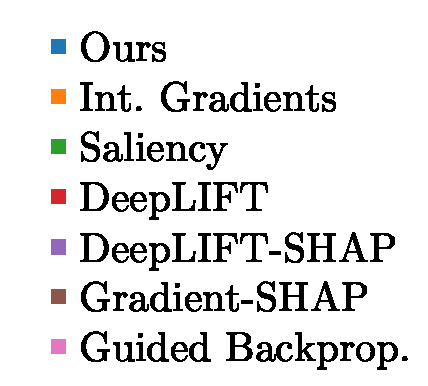
\includegraphics[scale=0.35]{../thesis/img/radar-legend.pdf}
        \end{subfigure}
    \end{figure}
\end{frame}

\begin{frame}
    \frametitle{Results}
    \framesubtitle{Quantitative (3/4)}
    
    \begin{figure}[H]
        \centering
        \begin{subfigure}[c]{0.3\linewidth}
            \centering
            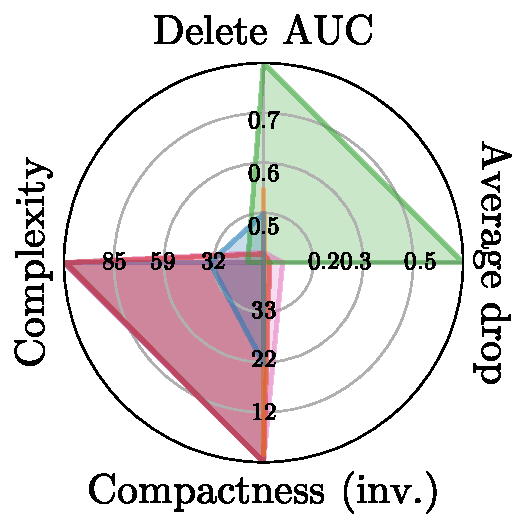
\includegraphics[width=0.9\linewidth]{../thesis/img/radar-mnist.pdf}
            \caption{MNIST}
        \end{subfigure}
        \begin{subfigure}[c]{0.3\linewidth}
            \centering
            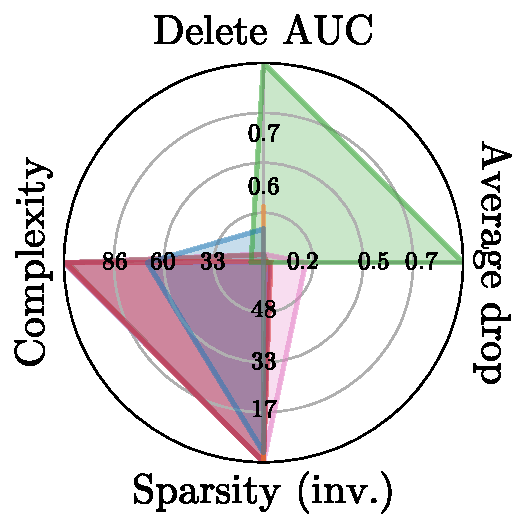
\includegraphics[width=0.9\linewidth]{../thesis/img/radar-cifar10.pdf}
            \caption{CIFAR-10}
        \end{subfigure}
        \begin{subfigure}[c]{0.3\linewidth}
            \centering
            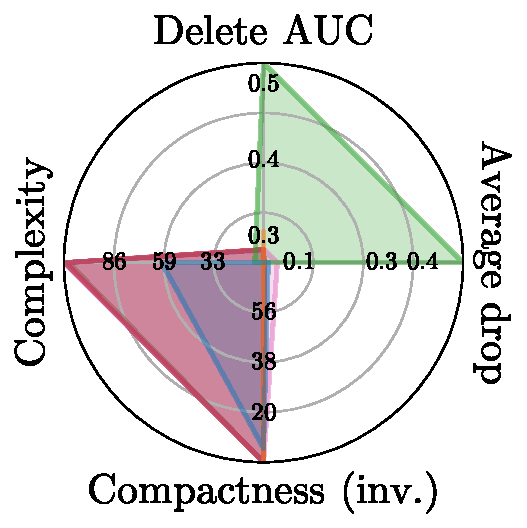
\includegraphics[width=0.9\linewidth]{../thesis/img/radar-imagenette.pdf}
            \caption{Imagenette}
        \end{subfigure}
        \begin{subfigure}[c]{0.2\linewidth}
            \centering
            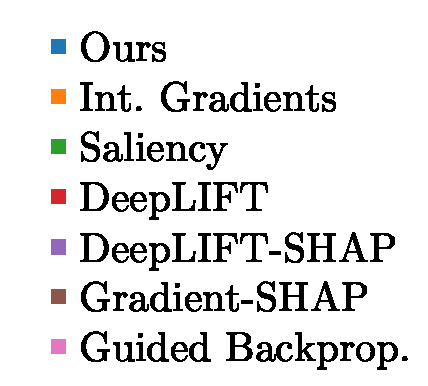
\includegraphics[scale=0.35]{../thesis/img/radar-legend.pdf}
        \end{subfigure}
    \end{figure}
\end{frame}

\begin{frame}
    \frametitle{Results}
    \framesubtitle{Quantitative (4/4)}
    
    \begin{figure}[H]
        \centering
        \begin{subfigure}[c]{0.3\linewidth}
            \centering
            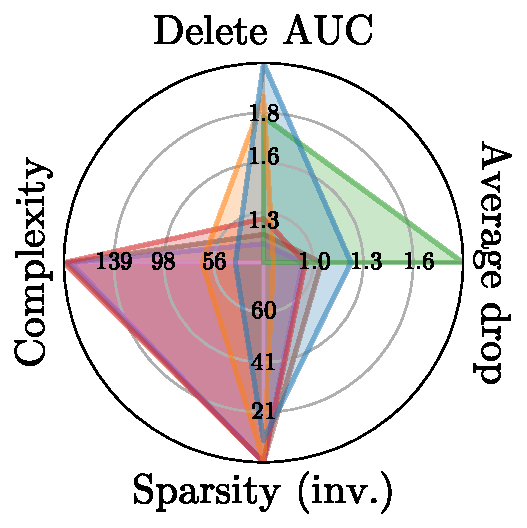
\includegraphics[width=0.9\linewidth]{../thesis/img/radar-flickr8k.pdf}
            \caption{Flickr8k}
        \end{subfigure}
        \begin{subfigure}[c]{0.3\linewidth}
            \centering
            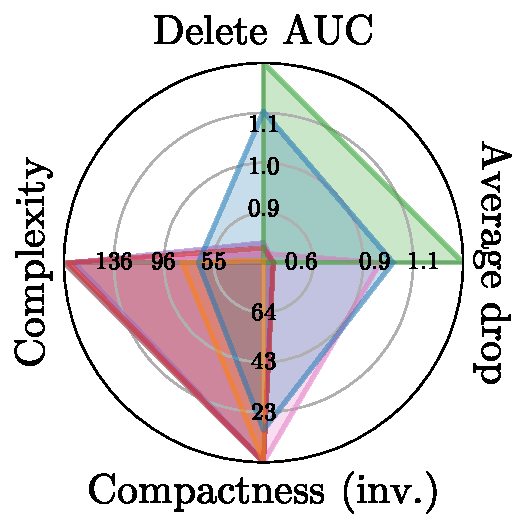
\includegraphics[width=0.9\linewidth]{../thesis/img/radar-hateful_memes.pdf}
            \caption{Hateful Memes}
        \end{subfigure}
        \begin{subfigure}[c]{0.3\linewidth}
            \centering
            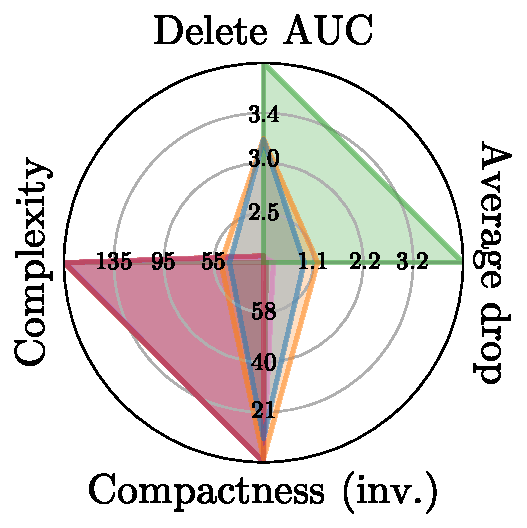
\includegraphics[width=0.9\linewidth]{../thesis/img/radar-snli_ve.pdf}
            \caption{SNLI-VE}
        \end{subfigure}
        \begin{subfigure}[c]{0.2\linewidth}
            \centering
            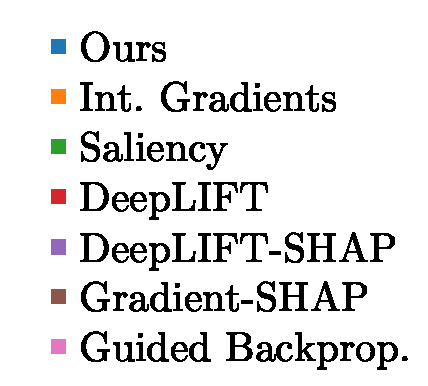
\includegraphics[scale=0.35]{../thesis/img/radar-legend.pdf}
        \end{subfigure}
    \end{figure}
\end{frame}


\begin{frame}
    \frametitle{Results}
    \framesubtitle{Qualitative}
    
    \begin{itemize}
        \item Saliency is the method that tends to assign high importance scores to a very small subset of the input space.
        \item The other baselines tend to give some degree of imporance to the whole input.
        \item Our method tend to only select a subset of the input as relevant.
    \end{itemize}
\end{frame}


\begin{frame}
    \frametitle{Results}
    \framesubtitle{Qualitative}

    \begin{figure}[H]
        \centering
        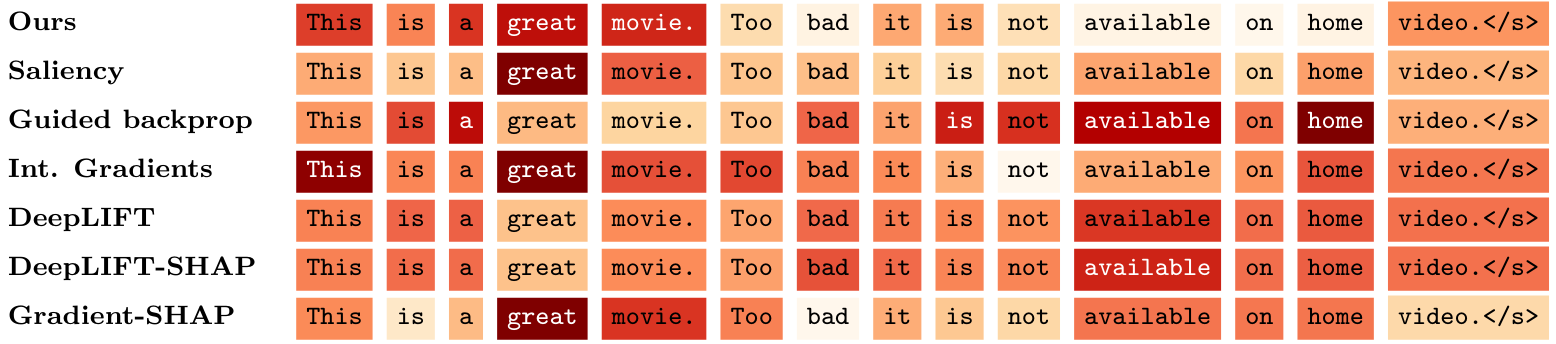
\includegraphics[width=\linewidth]{./img/text.png}
    \end{figure}

    \begin{figure}[H]
        \centering
        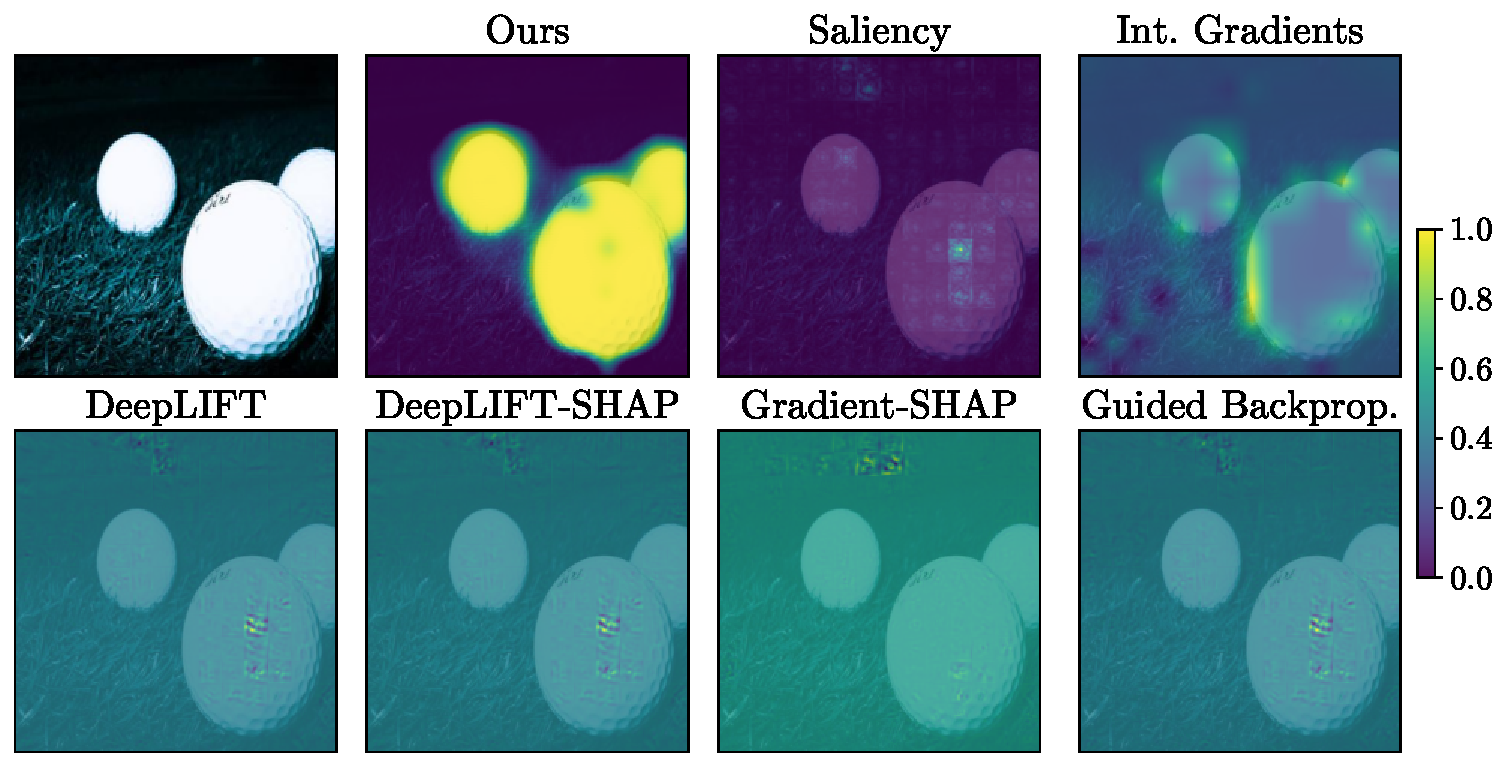
\includegraphics[width=0.7\linewidth]{../thesis/img/imagenette.pdf}
    \end{figure}
\end{frame}


\begin{frame}
    \frametitle{Results}
    \framesubtitle{Ablation study}

    \begin{itemize}
        \item Each design choice contributes to improve either faithfulness or clarity.
    \end{itemize}

    \begin{figure}[t!]
        \centering
        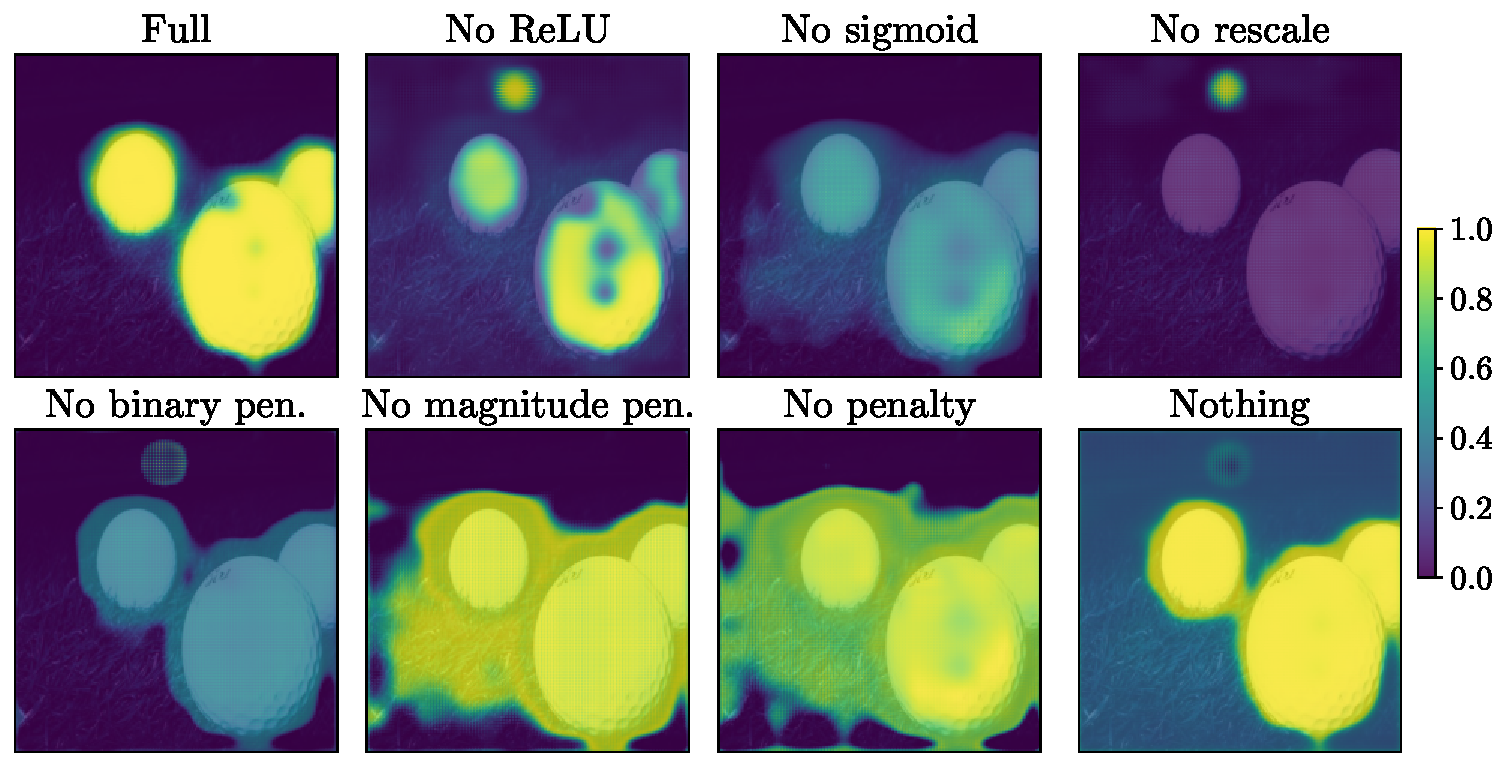
\includegraphics[width=0.85\linewidth]{../thesis/img/imagenette-ablation.pdf}
    \end{figure}
\end{frame}


\begin{frame}
    \frametitle{Conclusion}
    
    \begin{itemize}
        \item We proposed an attribution method that is trained in a self-supervised way, without introducing method-specific hyperparameters.
        \item We showed its applicability as a data-agnostic method for neural networks.
        \item We observed that among existing methods, ours has the best trade-off between model faithfulness and visual clarity both quantitatively and qualitatively.
    \end{itemize}
\end{frame}


\end{document}